\documentclass{EPL-master-thesis-covers-FR}

\title{HaïtiWater 2.0}
\subtitle{Evolution de l'application HaïtiWater vers une application entière  fonctionnelle hors-ligne}

\author{Vincent \textsc{Gradzielewski}}% Handcrafted third author :D

\degreetitle{Master [120] en sciences informatiques}

\supervisor{Kim \textsc{Mens}}
\secondsupervisor{Sandra \textsc{Soares-Frazão}}

\readerone{}
\readertwo{}

\years{2020-2021}

\usepackage{hyperref}
\usepackage{cite}
\usepackage{float}
\usepackage{multirow}
\usepackage{multicol}
\usepackage[final]{pdfpages}
\usepackage{booktabs}
\usepackage{multirow}
\usepackage{graphicx}
%\usepackage[toc]{multitoc}
%Vérifier la table des matière (une colonne)

\usepackage{amssymb}% http://ctan.org/pkg/amssymb
\usepackage{pifont}% http://ctan.org/pkg/pifont
\newcommand{\cmark}{\ding{51}}% pour les checkmark
\newcommand{\xmark}{\ding{55}}%

\frenchbsetup{StandardLists=true} % Resolves conflict between babel and enumitem
\usepackage{enumitem} % better formating of lists

\usepackage[style=long,nonumberlist,toc,xindy,acronym,nomain]{glossaries}
%Vé
\makenoidxglossaries
\input{../documents/requirements/glossary.gloss}

\begin{document}

	\maketitle
	\tableofcontents

	\setlength{\parskip}{1.5em plus1em minus1em}

	% Total des pages : entre 49 et 75 d'après nos estimations.

	\chapter*{Résumé}
	\addcontentsline{toc}{chapter}{Résumé}
	
		%Objectif, solution, évaluation
	
		Ce travail de fin d'études a été réalisé dans le cadre de mon Master en Sciences Informatiques à l'École Polytechnique de Louvain-la-neuve durant l'année académique 2020-2021.
		
		Dans ce mémoire je vais présenter mon travail qui consistait à reprendre l'application HaïtiWater développée précedemment par Adrien Hallet, Céline Deknop et Sebastien Strebelle qui a pour but "La gestion du réseau de distribution d'eau potable en Haïti". Le but étant de faire évoluer cette application pour que celle-ci soie entièrement
		
		
		 afin de la faire évoluer vers une application web qui serait entièrement utilisable \textbf{hors-ligne}.
		 
		Cette application a pour but "La gestion du réseau de distribution d'eau potable en Haïti". Je commencerai par une brève introduction sur le contexte Haitien et sur les raisons pour lesquels l'évolution de cette application était nécessaire. Ensuite je présenterai le principe des progressive weba app et pourquoi j'ai choisis d'utiliser cette technologie plûtot qu'une autre. Je présenterai ensuite la validation de l'application et les feedbacks que j'ai reçu des utilisateurs ainsi que les conséquence de cette validation sur l'application finale. Puis je concluerai par une liste des améliorations possibles.

		Tout le travail réalisé est disponible ici :

\begin{itemize}
	\item Github : \url{https://github.com/exavince/HaitiWater}
	\item Par l'UCL : \url{https://haitiwater.sipr.ucl.ac.be}
	\item En Haïti : \url{unknown}
\end{itemize}		

		Si vous désirez tester l'application, il suffit de vous rendre sur un des liens cité précedemment et de vous connecter à l'aide de l'uilisateur qui vous sera communiqué si vous en faite la demande. Ces données ne seront pas révélées ici car les données ne peuvent pas être modifiéés aléatoirement. 
		

	\chapter*{Remerciements}
	\addcontentsline{toc}{chapter}{Remerciements}

		

	%\printnoidxglossary[title=Glossaire, toctitle=Glossaire]
	%\glsaddall

	\chapter{Introduction}

		
		\subsection*{Contexte}
		
			Ce mémoire appartient à un projet de développement financé par ARES-CCD avec quelques partenaires tels que Protos\footnote{\href{https://www.protos.ngo/fr/}{www.protos.ngo}}, l'UCL et l'UEH. 
			
			protos est une ONG qui vise à améliorer l'accès à l'eau potable dans plusieurs pays du monde afin de les aider à se développer. 
			
			Suite à de nombreuses crises politiques et catastrophes naturelles qui ont détruit beaucoup d'infrastructures locales, l'accès à l'eau potables est devenu difficile en Haïti. De plus, des incertitudes politiques entravent la reconstruction de ces installations et les populations ne sont pas toujours aidées par les services publics pour assurer la distribution de l'eau. 
			
			Il y a quelques années Protos est entré en contact avec l'UCL afin de réaliser un système logiciel pilote pour la gestion de la distribution d'eau potable en zone rurale. C'est pour cette raison que l'ONG Protos est active dans le pays depuis quelques années et à permis aux anciens mémorants de créer l'application HaïtiWater.
			
			 En effet, aucune gestion centralisée organisée par l'Etat n'existe pour ces zones, éloignées des grandes agglomérations. Des réseaux existent, constitués de points de prélèvement d'eau, de conduites de distribution d'eau et de fontaines situées dans les villages, mais la gestion publique de ceux-ci n'est pas opérationnelle. 

			L'application créée précedemment propose un appui à ces organismes locaux afin de mieux organiser cette distribution. 
			%Explication de l'application des différents modules existants

			

		\subsection*{Problématiques}
		
			Actuellement l'application HaïtiWater est prévue pour fonctionner uniquement lorsque le réseau est stable et fonctionnel. Malheureusement en Haïti le réseau est assez instable et par endroit ce réseau n'est même pas disponible. La suite du développement de l'application va donc devoir porter sur le fonctionnement hors-ligne de celle-ci. 

			% Expliquer pourquoi l'application a besoin d'évoluer 

		\subsection*{Motivation}

			%Explqiuer pourquoi avoir choisis ce mémoire
			

		\subsection*{Objectifs}

			%Expliquer le but final du mémoire au niveau de l'usage de l'applcition en Haiti
			
		\subsection*{Approche}

			%Expliquer les différentes étapes par lesquelles je suis passé pour réaliser ce mémoire (étude des différentes tech, développement, validation, ...)
			
		\subsection*{Contribution}

			%Qu'est ce qu'a apporté le travail réalisé
			%Qu'elle est la plus value ?

		\subsection*{Plan}

			%Explication dans le temps des différentes phases de travail 

	\chapter{Contexte}


		\section{La gestion de l'eau en Haïti}
			\label{sec:situation}
			
				Haïti est l'un des pays les plus pauvres au monde. Le pays est situé dans une zone géographique où les risques de catastrope naturelle sont très éleves. Ces catastrophes détruisent les infrastructures et empêchent le bon développement des réseaux de distribution. Il y a quelques années, en 2010, le pays à subit un énorme séisme qui a ravagé une bonne partie du pays. Parmis tous les défis à relever viens celui de la gestion et de la distribution de l'eau potable sur le territoire, surtout dans les zones les plus rurales. Le climat de la région rendant excessivement difficle l'exploitation des cours d'eau, il faut beaucoup d'infrastructure afin de pouvoir exploiter l'eau potable.
				
				En raison de la grande pauvreté et de gros problèmes organisationnels qui règnent sur la plupart de l'île, il est très difficle de maintenir et de développer le réseau de distribution d'eau potable. Il y a un gros manque de collaboration entre les entités haïtiennes ou entre les villages dû en partie à la communication qui n'est pas du tout optimmisée voir inexistante dans certains cas. Dans les zones les plus rurales de l'île, le taux de recouvrement des factures est excessivement faible, jusqu'à 11\%.
				
				Pour toutes ces raisons, l'ONG Protos vient donc en aide à Haïti afin d'aider le service national des eaux à gérer la gestion des infrastructures et la facturation des clients surtout dans les zones rurales.
				
				Si vous désirez plus d'informations sur les problèmes environementaux, politiques, sociaux ou organisationnels du contexte haïtiens, je vous invite à aller consulter le mémoire d'Adrien Hallet, Céline Deknop et Sébastien Strebelle intitulé :
				"HaïtiWater, développement d'une application web pour gérer la distribution de l'eau en Haïti".

				%Brève explication sur le contexte Haïtien


		\section{Introduction à l'application}
				Dans le cadre de la situation décrite dans la section "Gestion de l'eau à Haïti, Protos a fait appel à l'UCL afin de créer une application d'aide à la gestion et la distribution de l'eau potable en Haïti. Une première version de l'application a été développée en 2018-2019 par 3 personnes dans le cadre de leur mémoire, elle comprend différents modules permettant de faciliter la gestion des infrastuctures et les clients qui vont y chercher de l'eau.
				
			\subsection{Utilisateurs}
				Il y 2 types d'utilisateurs qui peuvent se connecter à l'application : les gestionnaires de zone et les gestionnaires de fontaine. Ceux-ci ont des privilèges différents et peuvent donc intéragir différents avec les données.
				\begin{table}[H]
					\centering
					\small
					\setlength\tabcolsep{2pt}
					\begin{tabular}{|l|c|c|}
						\hline
						\multirow{2}{*}{\textbf{Permission}} & \multicolumn{2}{l|}{\textbf{Gestionnaire de}} \\ \cline{2-3}
						 & \textbf{fontaine} & \textbf{zone} \\ \hline
						 Ajouter/modifier/supprimer un consommateur & \cmark & \cmark \\ \hline
						 Ajouter/modifier/supprimer un élément du réseau de distribution & \cmark & \cmark \\ \hline
						 Ajouter/modifier/supprimer un rapport mensuel & \cmark & \cmark \\ \hline
						 Ajouter/modifier/supprimer un paiement & \cmark & \cmark \\ \hline
						 Ajouter/modifier/supprimer un ticket de support & \cmark & \cmark \\ \hline
						 Ajouter/modifier/supprimer une zone & \xmark & \cmark \\ \hline
						 Ajouter/modifier/supprimer un gestionnaire & \xmark & \cmark$^{*}$ \\ \hline
						 Accepter/refuser un changement dans l'historique & \xmark & \cmark \\ \hline
						 \multicolumn{3}{p{\textwidth}}{\emph{* : Un gestionnaire de zone ne peut pas modifier les informations personnelles (mot de passe, courriel, nom, prénom) d'un gestionnaire existant}} \\
					\end{tabular}
					\caption{Permissions dans l'application, par type d'utilisateur}
					\label{tab:permissions}
				\end{table}
				
			\subsection{Accueil}
				Ce module contient les informations condensées de la zone qui est attribuée à l'utilisateur. Il peut y retrouver le nombre de fontaines, de kiosques, de point de prises individuelles et de conduites que contient sa zone mais aussi le nombre de foyers et de consommateurs individuels de celle-ci. 
				
				Ce module n'est présent qu'à titre de présentation et de page d'accueil.
				
				\begin{figure}[H]
					\centering
					\includegraphics[width=1\textwidth]{images/Accueil}
					\caption{Module accueil}
				\end{figure}
				
				
			\subsection{Réseau}
				Dans ce module, l'utilisateur peut retrouver 3 éléments différents :
				\begin{itemize}
					\item En haut à gauche, une partie où il peut consulter le schéma de répartition des consommateurs par genre ou le volume d'eau mensuel distribué dans chaque zone. Il peut séleectionne le schéma a voir grâce à une liste déroulante.
					\item En haut à droite, une partie où il peut voir un résumé de sa zone géographique contenant le nombre de consommateurs et de points d'eau présent ainsi que le volume d'eau distribué dans celle-ci.
					\item En bas, un tableau intéractif qui contient tous les différents éléments du réseau. Dans cette partie en fonction des privilèges de l'utilisateur, celui-ci peut supprimer, modifier ou ajouter des éléments du réseau. Il peut également faire des recherche ou encore trier ce tableau selon ses besoins.
				\end{itemize}
				
				\begin{figure}[H]
					\centering
					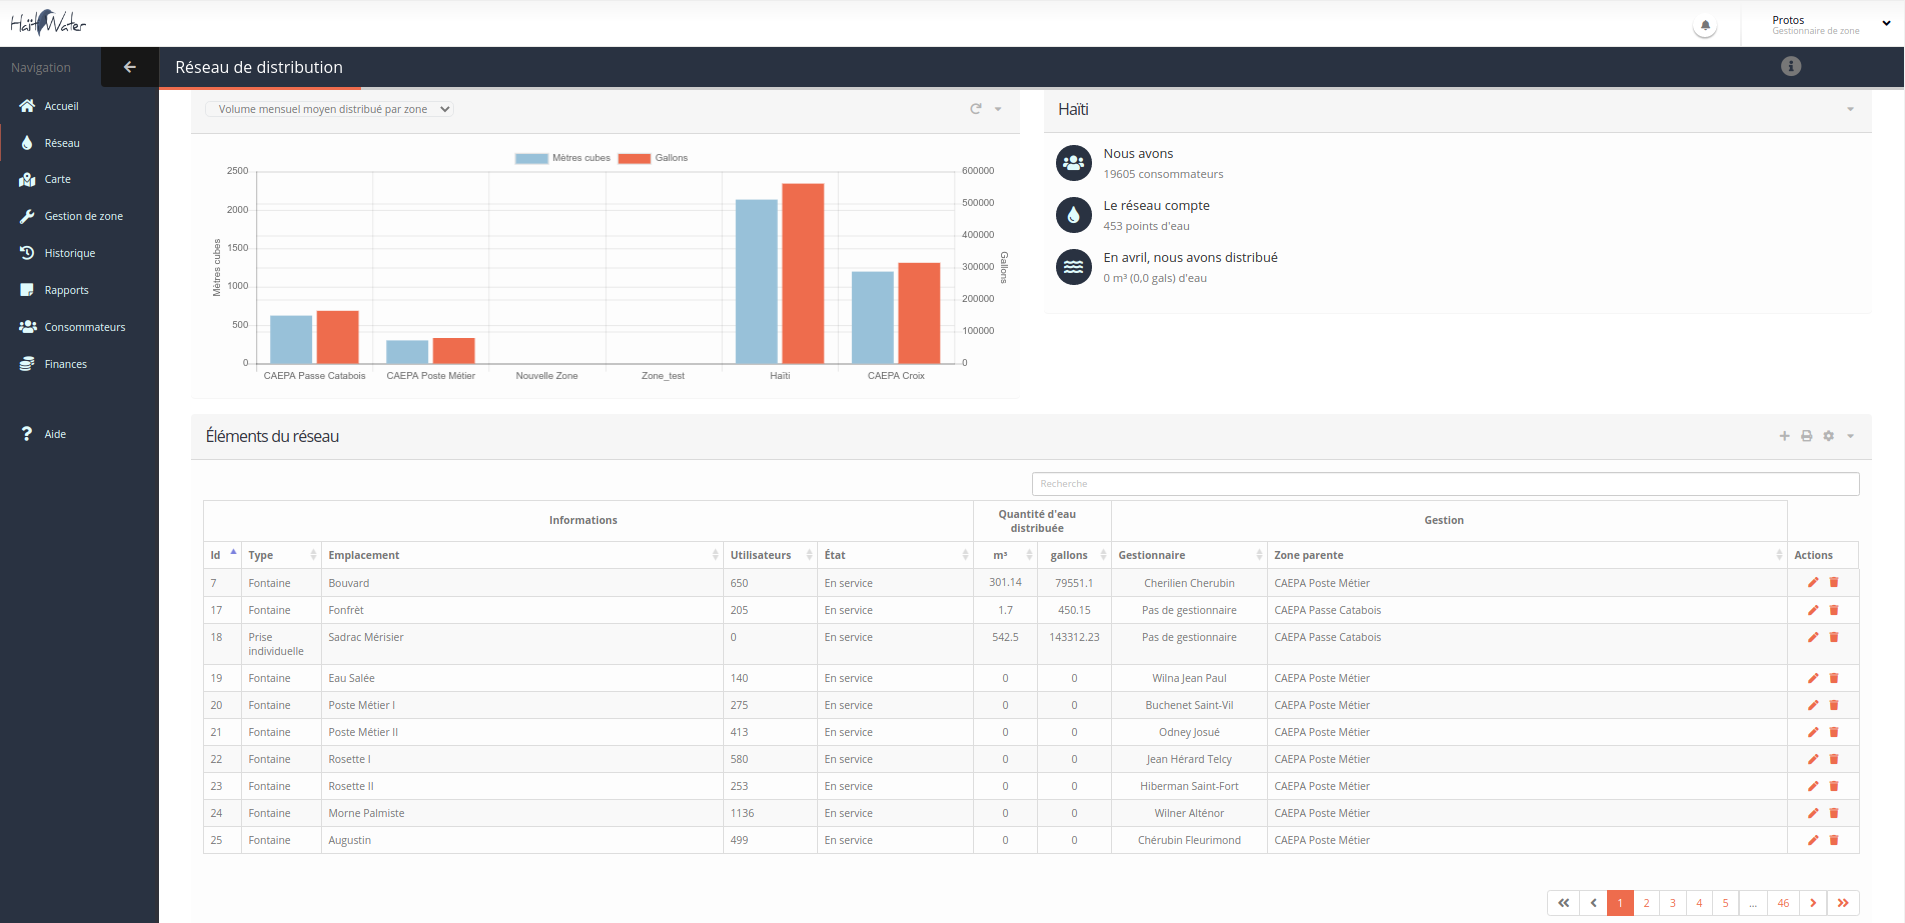
\includegraphics[width=1\textwidth]{images/reseau}
					\caption{Module réseau}
				\end{figure}
				
			\subsection{Carte}
				Ce module comprend un tableau réduit des éléments du réseau ainsi qu'une carte interactive qui permet à l'utilisateur de voir où sont situés les différents éléments du réseau et de connaître ou d'encoder les coordonnées géographiques de ceux-ci. Comme dans le module "réseau", il est également possible d'ajouter, modifier ou supprimer des éléments du réseau.
				\begin{figure}[H]
					\centering
					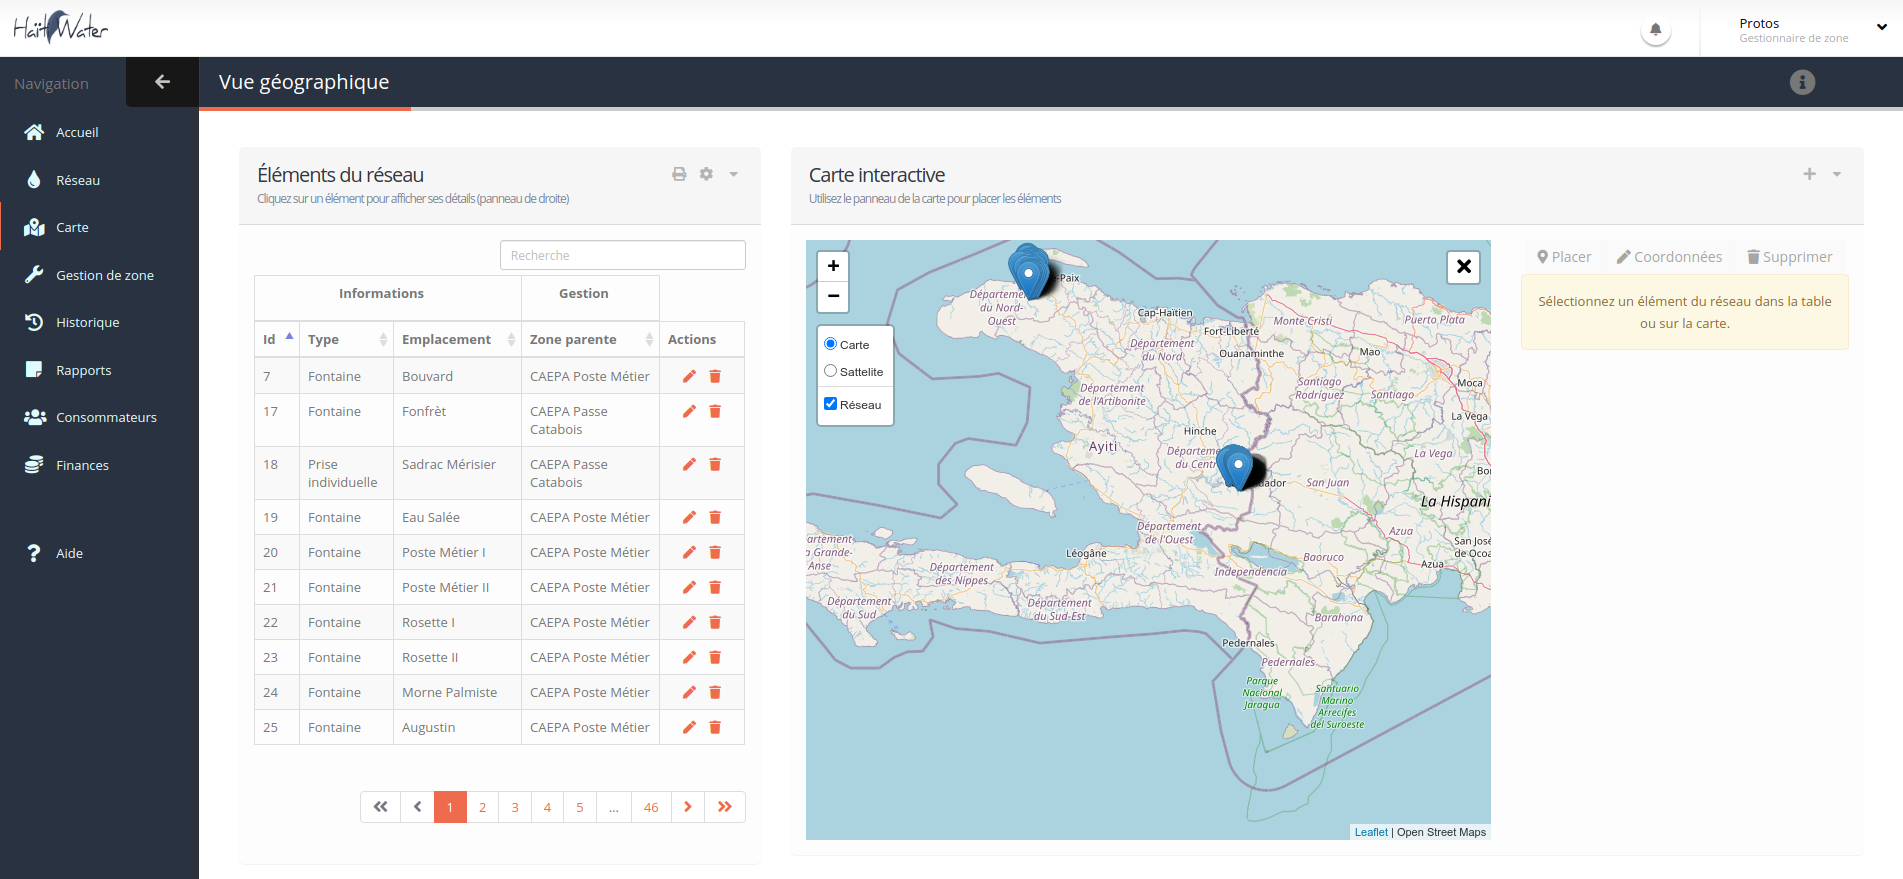
\includegraphics[width=1\textwidth]{images/carte}
					\caption{Mordule carte}
				\end{figure}
				
			\subsection{Gestion de zone}
				Ce module comprend 3 tableaux permettent à l'utilisateur de gérer sa zone :
				\begin{itemize}
					\item Le tableau en haut à gauche contient les différentes zones géographiques encodées dans le système. Cliquer sur un des éléments du tableau permet de filtrer les éléments des deux autres tableaux qui seront décris plus bàs afin de ne garder que les éléments de la zone concernée. Ce tableau permet également si l'utilisateur à les privilèges requis d'ajouter, supprimer ou modifier une zone.
					\item Le tableau en haut à droite contient la liste de tous les gestionnaires. Cliquer sur un gestionnaire permet à l' utilisateur de filtrer les éléments réseaux qui sont gérés par ce gestionnnaire. De nouveau si l'utilisateur possède les privilèges nécessaires vous pourrez ajouter, modifier ou supprimer des gestionnaires.
					\item Le dernier tableau contient le même tableau que la section réseau. L'utilisateur peut y faire tout ce qui a été décrit dans la section "Réseau".
				\end{itemize}
				\begin{figure}[H]
					\centering
					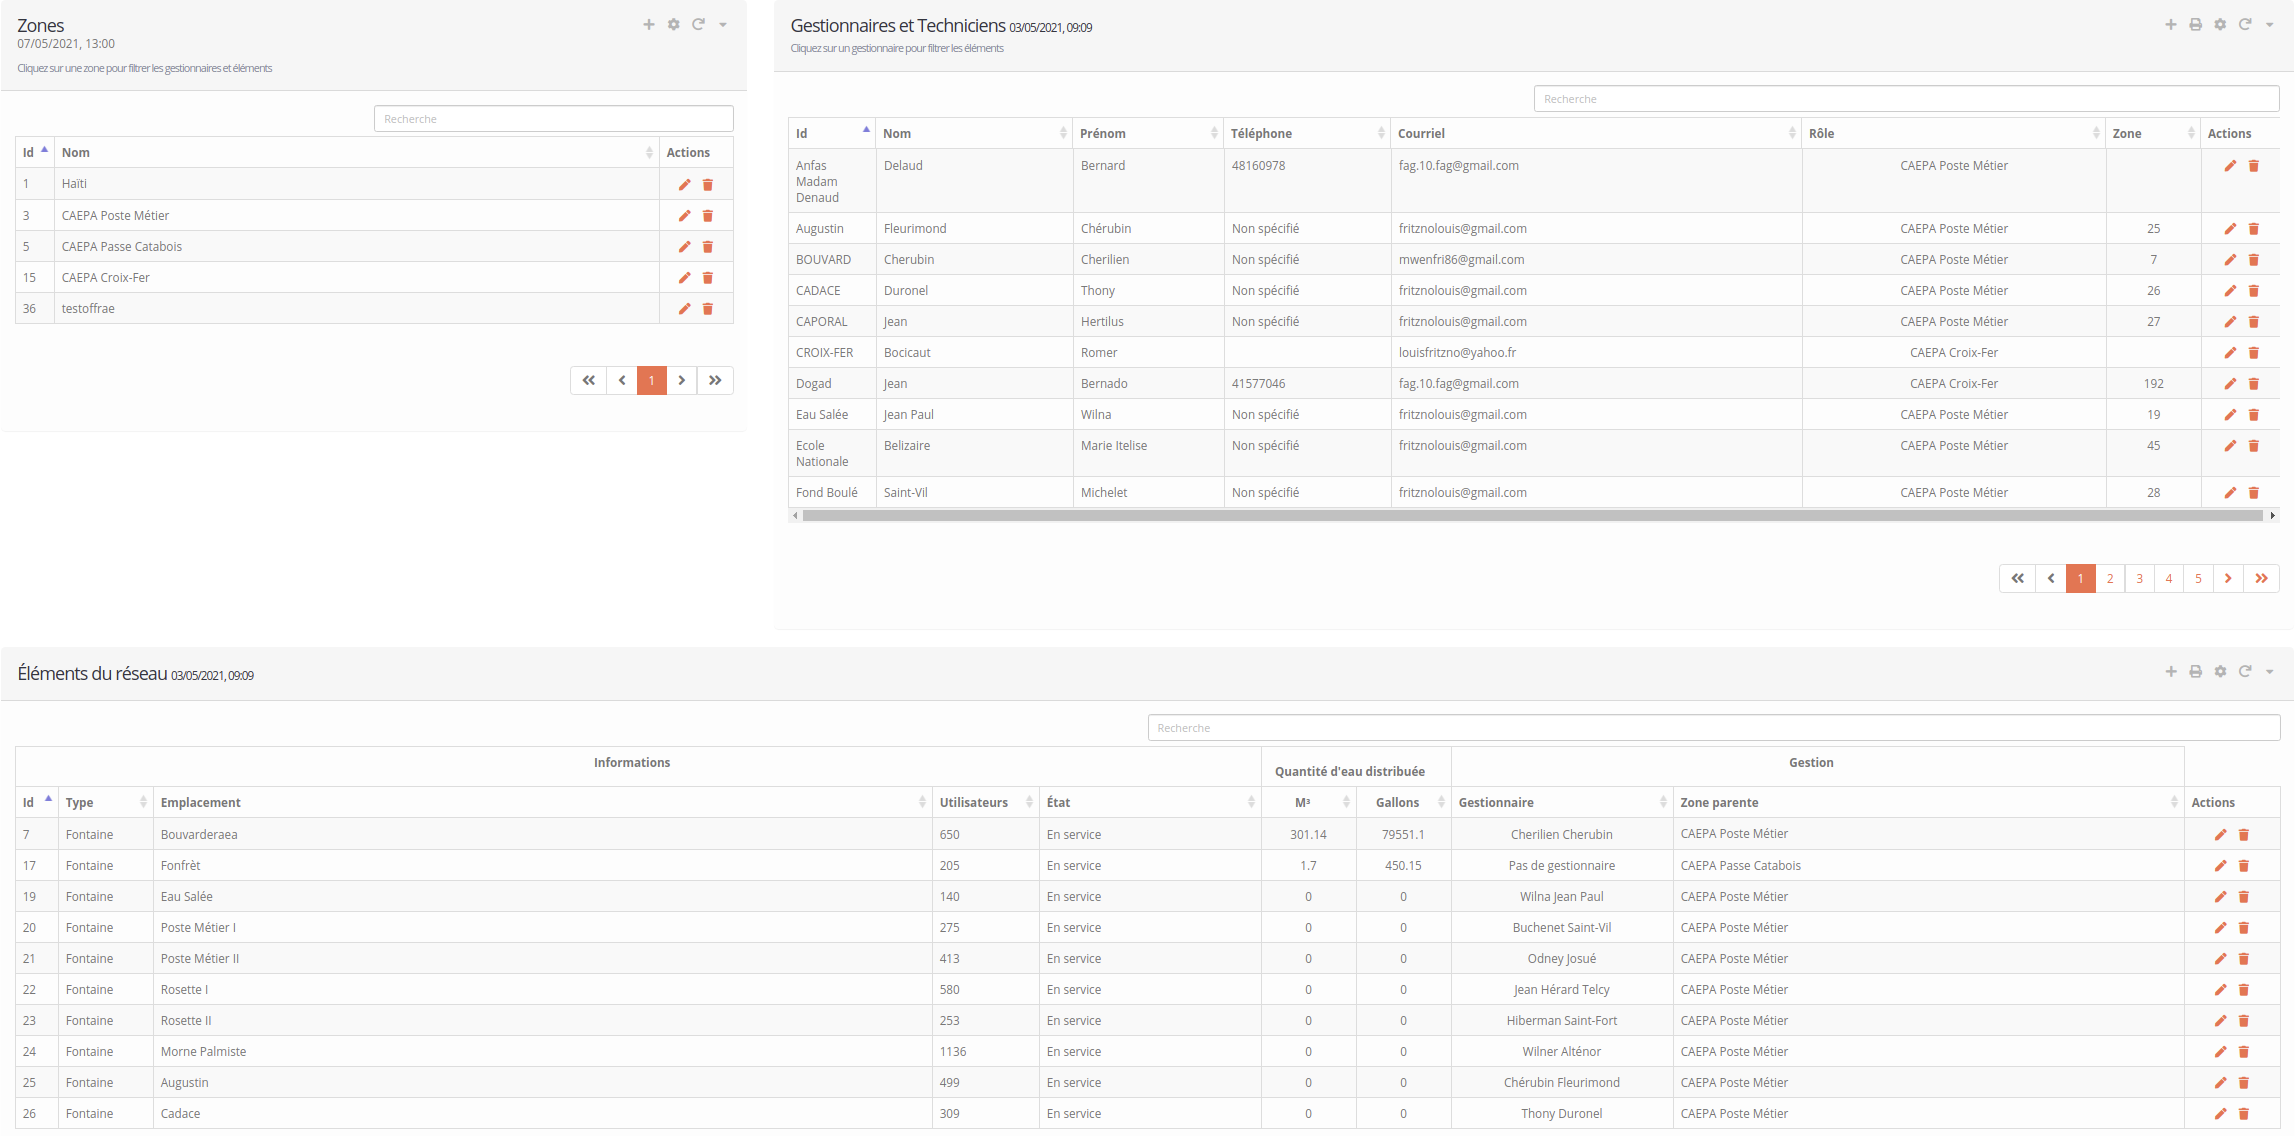
\includegraphics[width=1\textwidth]{images/gestion}
					\caption{Module gestion de zone}
				\end{figure}
			
			\subsection{Historique}
				Ce module contient les actions ayant été effectuées par des utilisateurs n'ayant pas tous les privilèges. Ces actions doivent être validées ou refusées par un gestionnaire plus haut placé. On peut y retrouver deux tableaux :
				\begin{itemize}
					\item Le tableau du haut contient les éléments devant être validés. Ici si l'utilisateur a les privilèges requis, vous pouvez choisier de confirmer ou non un action qui été encodée.
					\item Le tableau du bas contient les éléments qui ont été validés ou refusés dans les 3 dernières semaines. Il s'agit simplement d'un historique récent
				\end{itemize}
				\begin{figure}[H]
					\centering
					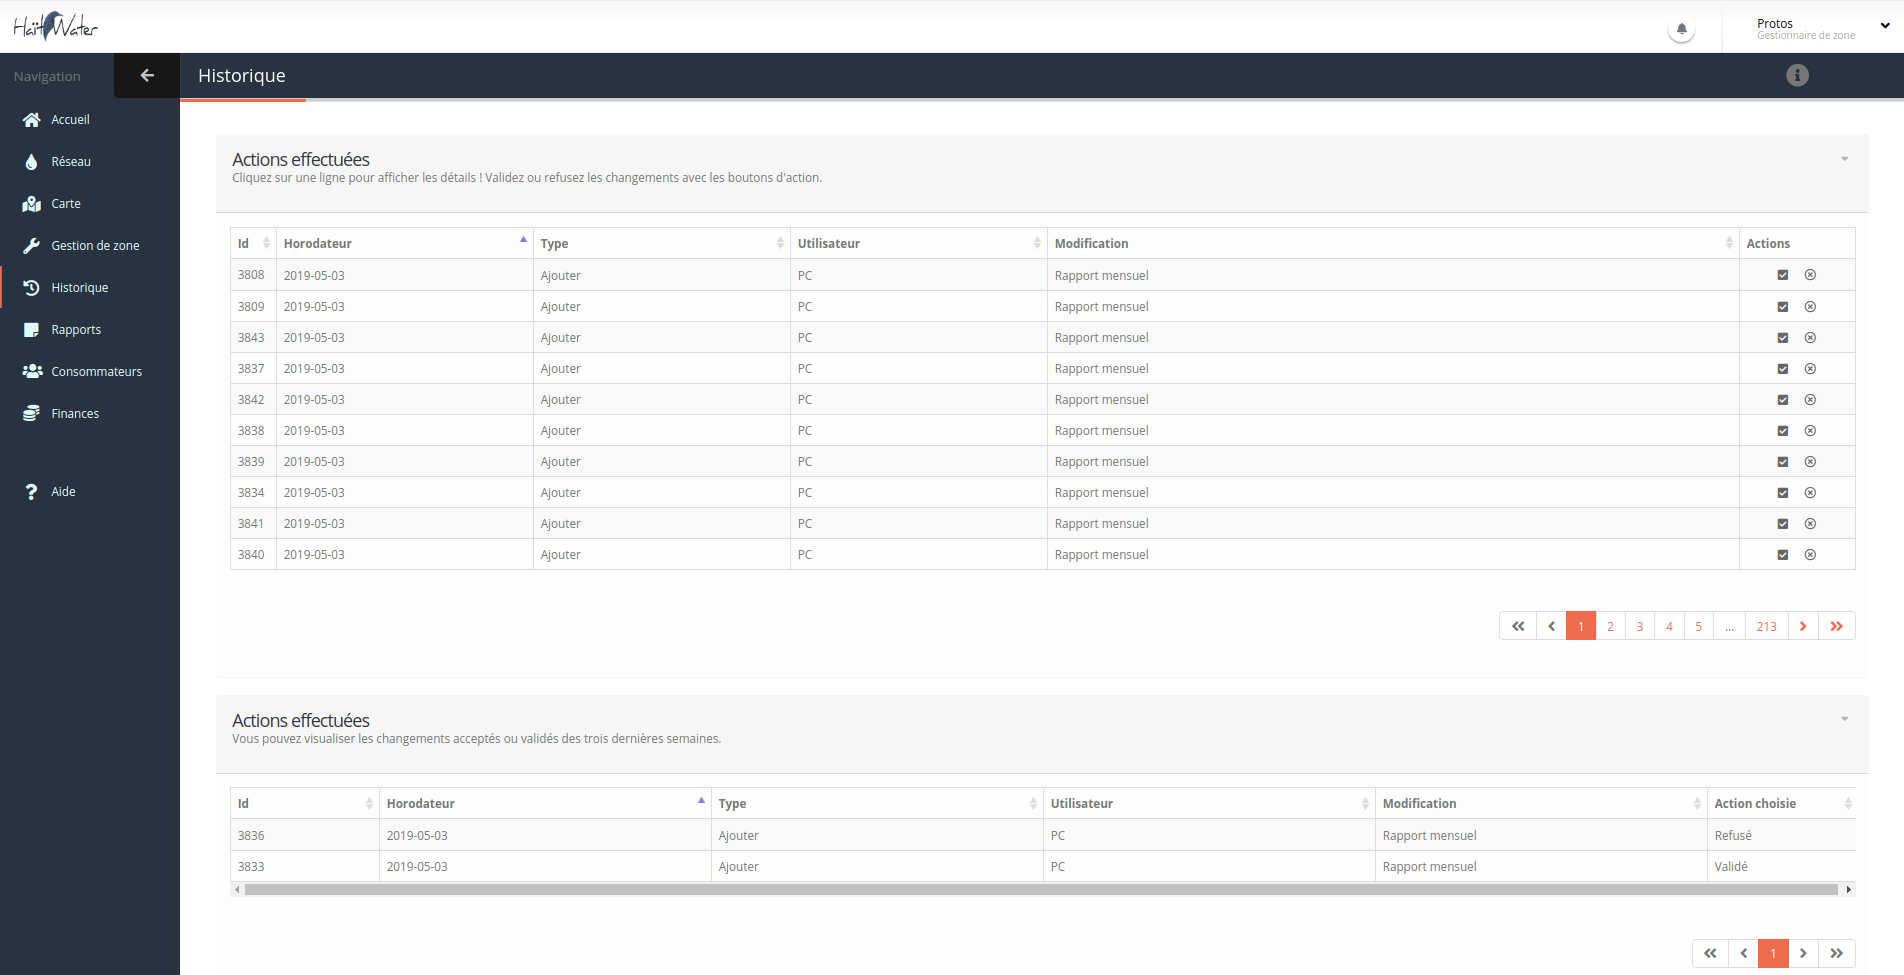
\includegraphics[width=1\textwidth]{images/historique}
					\caption{Module historique}
				\end{figure}
			
			\subsection{Rapports}
				Dans ce module, l'utilisateur peut signaler les différents problèmes qu'il rencontre avec les infrastructures de distribution d'eau. Une fois le problème signaler, celui-ci peut consulter ce qu'il a encodé dans le tableau juste en dessous et modifier ou supprimer son signalement. Si ses privilèges sont suffisament élevés, il pourra également gérer les signalements des autres personnes.
				
				C'est également ici que l'utilisateur va pouvoir encoder les rapports mensuels. Si jamais le réseau n'est plus présent, il pout simplement enregistrer le formulaire avec les données qu'il a encodée afin de l'envoyer plus tard lorsque le réseau sera de nouveau accessible.
				
				\begin{figure}[H]
					\centering
					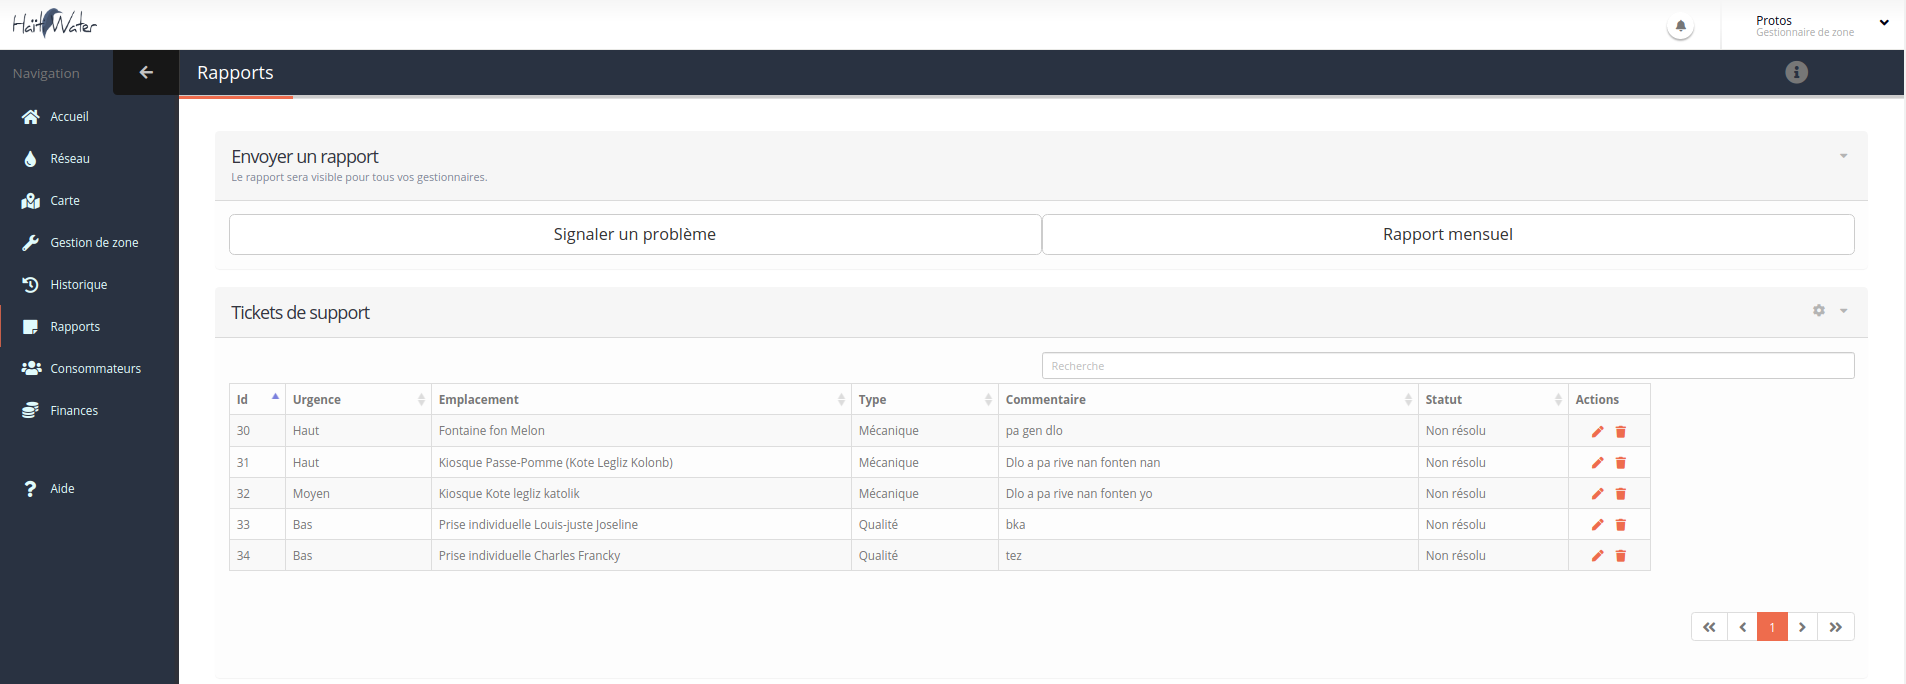
\includegraphics[width=1\textwidth]{images/rapport}
					\caption{Module rapport}
				\end{figure}
			
			\subsection{Consommateurs}
				Dans ce module, l'utilisateur retrouve 3 parties différentes :
				\begin{itemize}
					\item En haut à gauche vous pouvez afficher les mêmes schémas que ceux disponible dans la section "réseau".
					\item La partie en haut à droite contient un résumé de la situation de votre zone (nombre de foyer consommant de l'eau, nombre de consommateur, nombre de foyer n'ayant pas payé leur facture).
					\item Dans le bas on retrouve un tableau qui reprend tous les consommateurs auquels l'utilisateur à accès. Avec les bons privilèges, celui-ci peut ajouter, modifier ou supprimer des consommateurs. Ou bien il peut également juste consulter tous les détails sur les différents consommateurs.
				\end{itemize}
				
				\begin{figure}[H]
					\centering
					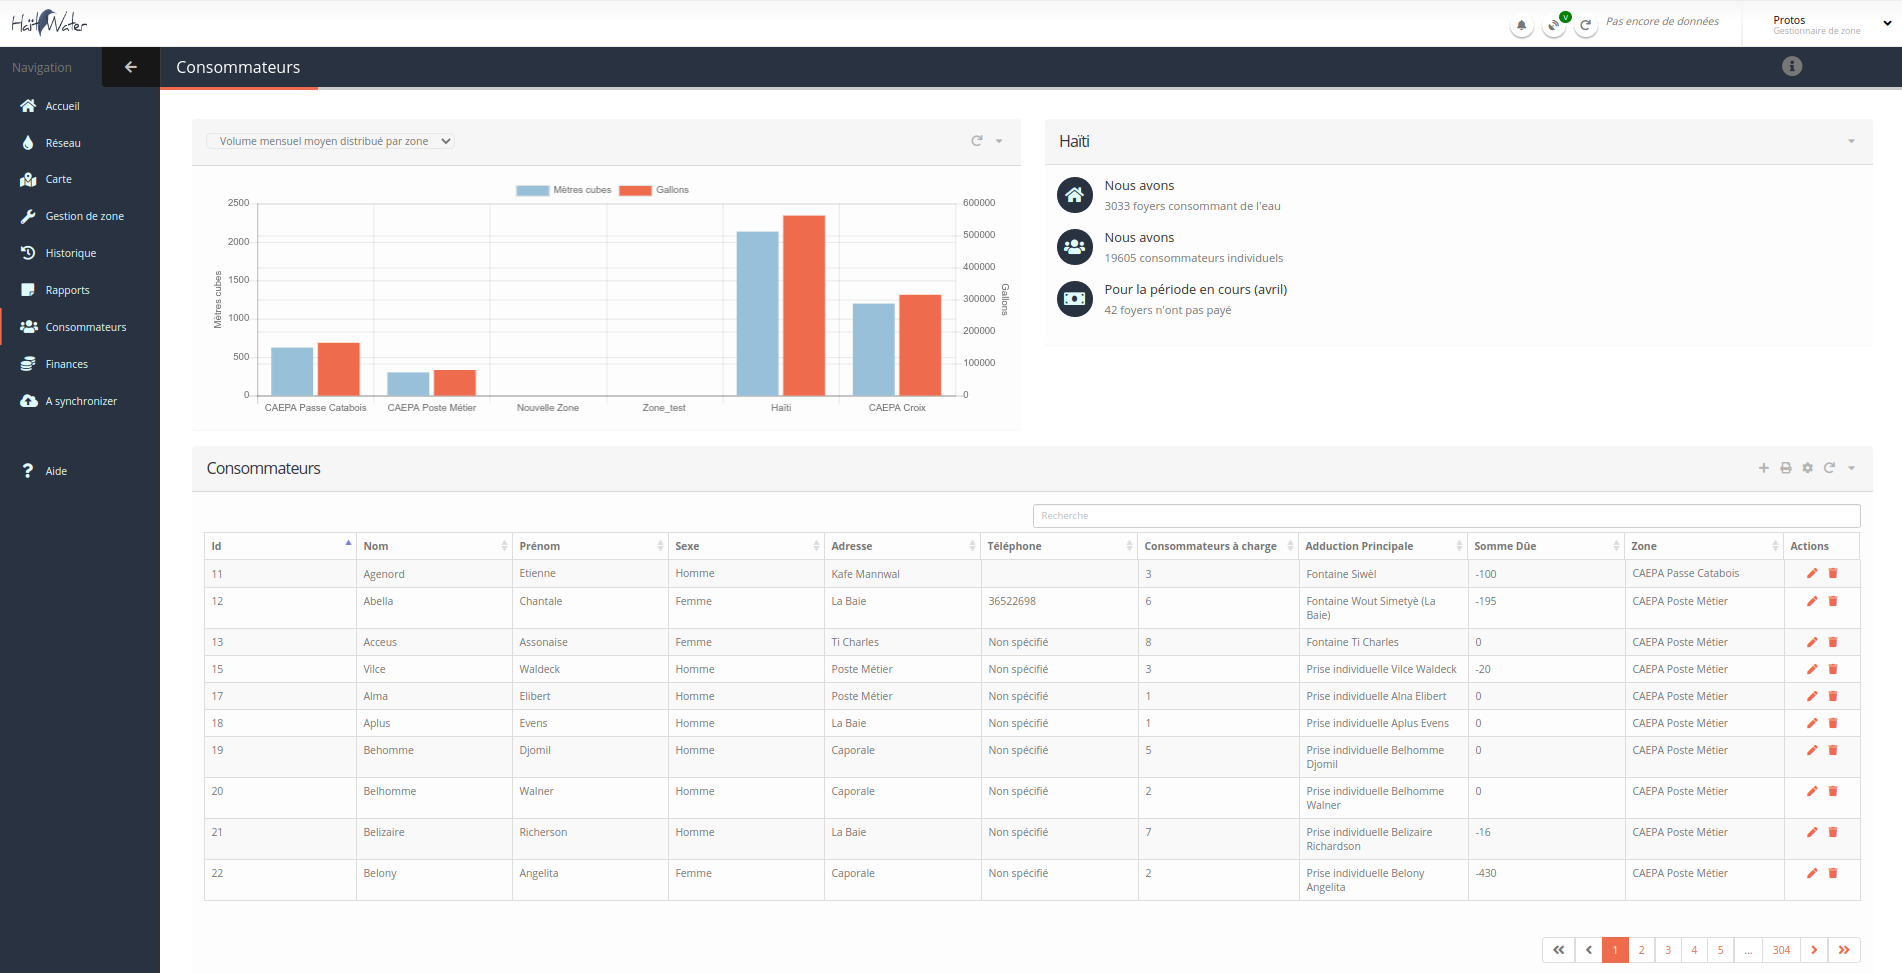
\includegraphics[width=1\textwidth]{images/consommateurs}
					\caption{Module consommateurs}
				\end{figure}
			
			\subsection{Finances}
				Dans ce module, l'utilisateur a accès à 4 tableaux différents qui lui permettent de gérer les finances de ses consommateurs. En fonction de ses privilèges, celui-ci pourra modifier, supprimer ou ajouter des informations dans les différents tableaux
				\begin{itemize}
					\item En haut à gauche, un tableau contenant les différentes zones. Le fait de sélectioner une zone permet à l'utilisateur de filtrer les consommateurs en fonction de leur zone d'attribution.
					\item En haut à droite, un tableau contenant les consommateurs auxquels l'utilisateur a accès. Le fait de sélectionner un consommateur permet de faire apparaître les deux tableaux suivants.
					\item En bas à droite, un tableau contenant les coordonnées du consommateur sélectionné ainsi que la somme dûe par celui-ci. Il n'est pas possible de modifier des données manuellements dans ce tableau.
					\item En bas à gauche, s'affiche tous les paiements effectués par le consommateur sélectionné. Ici l'utilisateur peut ajouter, modifier ou supprimer des paiements.
				\end{itemize}
				
				\begin{figure}[H]
					\centering
					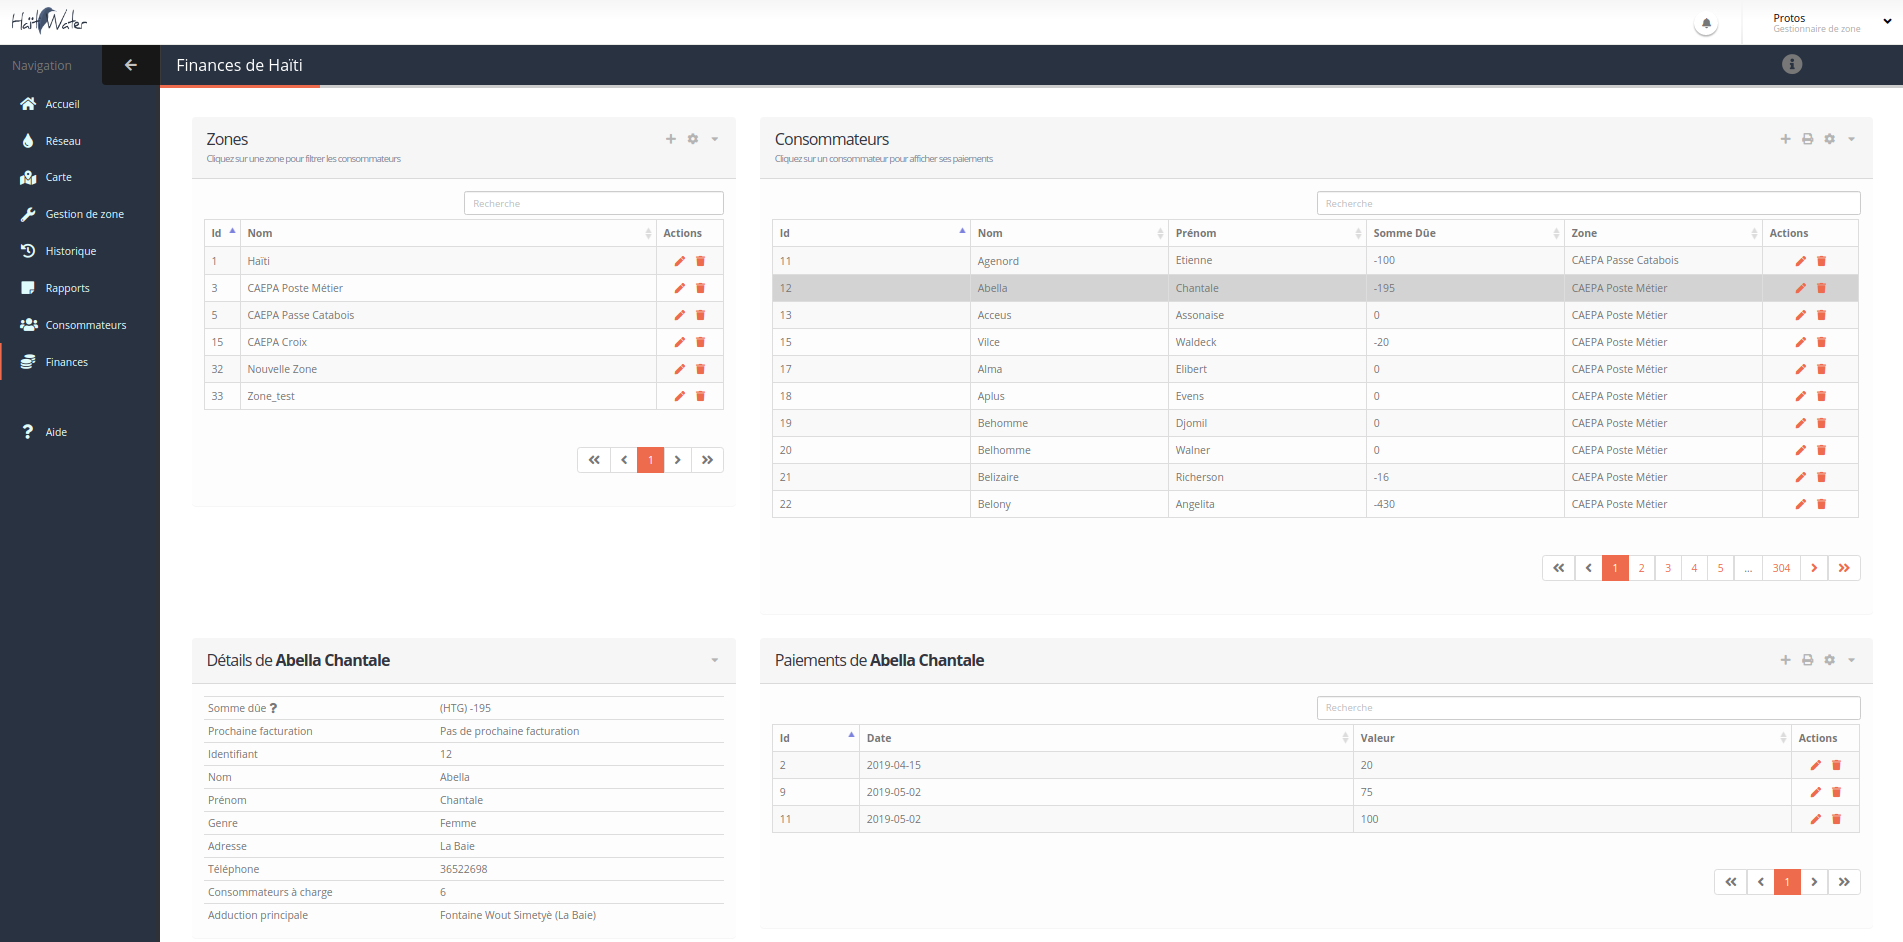
\includegraphics[width=1\textwidth]{images/finances}
					\caption{Module finances}
				\end{figure}
				
				
				
\newpage
		\section{Problèmes réseaux}
			L'application HaïtiWater est une application web classique. Cela signifie que pour fonctionner, il faut qu'il y ai nécessairement du réseau. Hors en Haïti, le réseau n'est pas très stable en ville et celui-ci peut aller jusqu'à être inexistant lorsque vous vous aventurez dans les zones les plus rurales. 
			
			Ces problèmes de connexions font que l'application est difficilement utilisable sur le terrain en toute sérénité car on ne sait jamais quand le réseau va devenir capricieux. Pour palier à ce problème, il a été décidé de transformer l'application web existante pour que celle-ci puisse fonctionner même lorsque le réseau est absent.
				
			De part sa nature, une application web nécessite un connexion pour pouvoir fonctionner. Il a donc fallu étudier les différentes options qui pourrait permettre de faire fonctionner l'application hors-ligne. Parmis les ces options,  les deux qui ont été retenues étaient de soit créer une \textbf{application mobile} séparée de l'application web, soit de transformer l'application web existante en \textbf{Progressive Web App}. 
				
			L'avantage de créer une application dédiées aux mobiles est qu'il est très simple de gérer le fonctionnement hors-ligne de cette application. De plus on peut plus facilement utiliser les différentes capacités de l'appareil mobile comme la caméra, la localisation, ...
			L'inconvénient de cette solution est qu'il fallait du coup générer une nouvelle application de A à Z. De plus cela implique qu'il y aura deux codes différents dans deux langages différents à devoir maintenir.
				
			L'avantage de la Progressive Web App est que tout se joue au niveau du navigateur. Il n'est donc pas nécessaire de devoir maintenir un deuxième code source. De plus aucune installation n'est nécessaire de la part de l'utilisateur et les mises à jour de l'application sont faites de manière transparante.
			L'inconvénient de cette solution est que la gestion du mode hors-ligne est un peu plus complexe, on ne peut pas profiter des capacités de l'appareil mobile aussi bien qu'avec une application native et cette technologie étant assez récente, il n'y a pas énormément de ressource d'aide en ligne et tous les navigateurs ne prennent pas en charge toutes les fonctionnalités proposées.
				
			Au vu de la situation compliquée en Haïti et du temps qui sera alloué à ce mémoire, il a été décidé que la meilleure option était celle de la Progressive Web App. La raison principale est qu'il aurait difficile une fois le mémoire terminé d'avoir deux codes sources différents à maintenir et à mettre à jour.

	\chapter{Organisation}
		

		Etant le seul étudiant à réaliser ce mémoire, il n'a pas été nécessaire d'utiliser des outils de plannification complets. Cette section contiendra surtout la plannification des différentes tâches à accomplir permettant l'aboutissement de l'application ainsi que l'écriture de ce mémoire. Celles-ci ont été mises place grâce aux discussions avec mes deux promoteurs et une étudiante en informatique venue d'Haïti pour en apprendre plus sur l'application. 

		\section{Approche de travail}
			Comprendre les enjeux et les différentes problématiques a été la première tâche à accomplir. Il a fallut décider du type de technologie à utiliser afin d'apporter les fonctionnalités nécessaires au bon fonctionnement de l'application. 
			
			La meilleure option aurait été de pouvoir en discuter avec la plupart des acteurs en Haïti afin d'avoir le plus d'avis possible sur la question. Mais vu le temps que cela aurait pris cette option n'était pas du tout envisageable. Pour pallier à se problème, nous avons étudié la question avec mes deux promoteurs et Nahomie l'étudiante venue d'Haïti. Celle-ci à pu nous apporter son expertise afin de choisir l'option idéale.
			
			Une fois le choix technologique fait, nous avons effectuer la plannification des tâches.
		
		

			%Etude du problème
			%Prioritisation des taches

			\subsection*{Planification}
				\label{sec:planification}

				%Planification des taches sur toutes l'année (reprendre planning développé pour le Q2)
		\section{Méthodologie}

			%Mise en place d'une méthode pour garantir l'avancement du projet

			\subsection*{Agile}
			
				%Pourquoi une méthode agile non fixe plutot que waterfall

				%Dev par fonctionnalité
				%Itération 
				

			\subsection*{Phases du mémoire}

			

	\chapter{Analyse des besoins}
		\label{sec:analyse_besoins}

		% Phase essentiele blabla
		% Retouver les schémas créé début d'année

		\section{Besoins fonctionnels}

			
			%éfinition

			\subsection*{Gestion des données}
				\label{sec:gest_donnee}



			\subsection*{Affichage et accès}

			

		\section{Besoins non-fonctionnels}

			%Définition

			\subsection*{Sécurité des données}


			\subsection*{Multi-plateforme}
				

			\subsection*{Technologies simples et populaires}


		\section{Structure modulaire}
			\label{sec:modules}

			%Expliquer que mon travail conserve la structure modulaire
			%Fin du module offline
			%Lien vers ancien mémoire
			%Ajout du module "A modifier"

			

		\section{Structure des données hors-ligne}
			\label{sec:data}

			%Expliquer la différence entre données online/offline
			%Introduire ma solution

	\chapter{Implémentation}

		\section{Description de l'app de base}
			%Expliquer l'implémentation de l'app existante
				%Django
				%PostGres
				%...
		
		\section{Choix technologiques}
			\label{sec:choix_tech}
			
			\subsection*{Progressive Web-App}
				%Expliquer les différentes types d'application hors-ligne étudiée
				
			\subsection{Stratégie de synchronisation des pages}			
			
			\subsection{Stratégie de synchronisation de la DB}
			
			
			\subsection{Gestion des changements d'utilisateurs}		
			
			
			\subsection{Sytème de notification}	
						

			\subsection*{Service-worker}

		
			\subsection*{IndexedDB}

					

			\subsection*{Dexie.js}
				

			\subsection*{DataTables}

			

			\subsection*{Chart.JS}
				
				

		\section{La hiérarchie dans l'application}
			%Epliquer qu'il y a eu ou pas des changements dans le fonctionnement de l'application au niveau des modules et de la hiérachie


			\subsection*{Structure}

			

			\subsection*{Permissions}

			

		\section{Interface utilisateur}
			%Expliquer les changements faits par rapport à l'interface de base
			%Ajout de couleurs, notifications, données non-sync, ...

		\section{Client}

			%Introduction

			\subsection*{Mise en cache}
				\label{sec:cache_client}

			
			\subsection*{Gestion des données}
				Gabarits, modularité et réactivité

			\subsection*{Push des données hors-ligne}
				\label{sec:service_worker}
				
				

			

		\section{Serveur}
			\label{sec:serveur}

		

			\subsection*{Requêtes}

			

			\subsection*{Détails des requêtes API}
				\label{sec:api}

			

	\chapter{Validation}

		%Introduction

		\section{Vérifications automatiques}

			\subsection*{Tests unitaires}

			

		\section{Vérifications utilisateurs réels}


			\subsection*{Méthodologie}

				

			\subsection*{Résultats obtenus}

				

			\subsection*{Modifications apportées}

		

	\chapter{Améliorations futures}


		\section{Suite du projet}
			\label{ref:suite_projet}

		

		\section{Défis rencontrés}

			

		\section{Propositions}

			
	\chapter{Conclusion}

		

		\section{Métriques}
		

	\bibliography{bibliography}{}
	\bibliographystyle{plain}
	\addcontentsline{toc}{chapter}{Bibliographie}
		

	

	\setlength{\parskip}{0em}
	\backcoverpage

\end{document}
